\documentclass[letterpaper, 10pt, conference]{ieeeconf}
\IEEEoverridecommandlockouts
% The preceding line is only needed to identify funding in the first footnote. If that is unneeded, please comment it out.

\let\proof\relax \let\endproof\relax


\usepackage{cite}
\usepackage{amsmath,amssymb,amsfonts}

\usepackage{graphicx}
\usepackage{textcomp}
\usepackage{xcolor}
\usepackage{amsmath, amssymb, amsthm}
\usepackage{algorithm}
\usepackage{algpseudocode}
\usepackage{booktabs}
\usepackage{hyperref}
\newtheorem{lemma}{Lemma}
\newtheorem{proposition}{Proposition}
\newtheorem{corollary}{Corollary}
\newtheorem{theorem}{Theorem}
\newtheorem{example}{example}
\newtheorem{remark}{Remark}
\newtheorem{assumption}{Assumption}
\newtheorem{definition}{Definition}
%\def\BibTeX{{\rm B\kern-.05em{\sc i\kern-.025em b}\kern-.08em
%    T\kern-.1667em\lower.7ex\hbox{E}\kern-.125emX}}
\begin{document}

% For draft editing
\newcommand{\Red}[1]{\textcolor{red}{[{#1}]}}

\title{\LARGE \bf
An Evolutionary Algorithm for Actuator-Sensor-Communication Co-Design in Distributed Control
}
\author{Pengyang Wu and Jing Shuang (Lisa) Li% <-this % stops a space
\thanks{At the time this manuscript was written, P.W. and J.S.L. were both with the Department of Electrical Engineering and Computer Science, University of Michigan, Ann Arbor, MI, 48109, USA.
        {\tt\small \{pengyanw, jslisali\}@umich.edu}.    }%
}

\maketitle

\begin{abstract}
This paper studies the co-design of actuators, sensors, and communication in the distributed setting, where a networked plant is partitioned into subsystems each equipped with a sub-controller interacting with other sub-controllers. The objective is to jointly minimize control cost (measured by LQ cost) and material cost (measured by the number of actuators, sensors, and communication links used). We approach this using an evolutionary algorithm to selectively prune a baseline dense LQR controller. We provide convergence and stability analyses for this algorithm. For unstable plants, controller pruning is more likely to induce instability; we provide an algorithm modification to address this. The proposed methods is validated in simulations. One key result is that co-design of a 98-state swing equation model can be done on a standard laptop in seconds; the co-design outperforms naive controller pruning by over 50\%.
\end{abstract}

\section{Introduction \& Motivation}
Large-scale networked dynamical systems arise in a wide range of modern engineering applications, including power grids, traffic networks, multi-agent robotic systems, and cyber-physical infrastructures. In such systems, centralized control architectures are often impractical due to scalability limitations and communication constraints. These challenges have motivated extensive research on \emph{distributed control}, where control actions are computed using only local information and limited inter-agent communication \cite{9535262, anderson2019system, shin}. There is also increasing interest in \emph{co-design} methodologies that jointly consider control performance, sensor and actuator placement, and communication structure. In the distributed control setting, co-design remains a fundamentally difficult problem, often translating to nonlinear mixed-integer programming problems (NLMIPs) or other similarly combinatorial problems. Existing approaches often focus on special subsets of the co-design problem which can be reduced to a more tractable form \cite{Pequito2015, Jiang2016, Moothedath2019, Singh2021}. However, this reduction eliminates large portions of the design space, which may contain more cost-effective solutions. 

In this paper, we study the co-design of actuators, sensors, and communication in the distributed linear-quadratic (LQ) setting via evolutionary algorithms (EA). EAs are heuristic optimization methods inspired by natural selection, and have demonstrated efficacy on complex problems such as NLMIPs \cite{Whitley2001, DeJong2014}. The problem setup is provided in Section \ref{sec:problem_setup}; the EA approach is described in Section \ref{sec:ea}. We then provide convergence (Section \ref{sec:convergence}) and stability (Section \ref{sec:stability}) analysis, as well as an additional sparsity-promoting modification to the base EA (Section \ref{sec:gersh_repair}); our approach and analyses are validated in simulation (Section \ref{sec:simulations}).

\section{Problem setup} \label{sec:problem_setup}

Consider a discrete-time linear time-invariant system:
\begin{equation} \label{eq:plant}
x_{k+1} = A x_k + B u_k
\end{equation}
where $x_k \in \mathbb{R}^{N_x}$ is the state vector, $u_k \in \mathbb{R}^{N_u}$ is the control input, $A \in \mathbb{R}^{N_x \times N_x}$ is the state matrix, and $B \in \mathbb{R}^{N_x \times N_u}$ is the input matrix. The system contains $N$ interconnected subsystems, each having one or more states. State and control are partitioned into $[x]_i$, $[u]_i$, and $[w]_i$ for each subsystem $i$; system matrices $A$ and $B$ are partitioned into $[A]_{ij}$, $[B]_{ij}$, which capture subsystem-level interaction. System topology is described by an unweighted directed graph $\mathcal{G}(\mathcal{V}, \mathcal{E})$, where vertex $v_i$ corresponds to subsystem $i$, and edge $e_{ij} \in \mathcal{E}$ exists whenever $[A]_{ij} \neq 0$ or $[B]_{ij} \neq 0$. Let $\mathcal{A}\in \{0,1\}^{N \times N}$ be the adjacency matrix for this graph, where by convention $\mathcal{A}_{ii} = 0$. For a state-feedback controller $u_k = Kx_k$, we can also partition $K$ into subsystems. Here, row $[K]_{i,:}$ is the sub-controller at subsystem $i$, and $[K]_{ij}$ represents information required by sub-controller $i$ from sub-controller $j$. We can similarly build a controller adjacency matrix $\mathcal{K}(K)$, where $\mathcal{K}(K)_{ij} = 1$ wherever $[K]_{ij} \neq 0$, and $\mathcal{K}_{ii} = 0$ by convention. 

The number of actuators used by the controller is $N_a(K) := \|K\|_{1,0}$, i.e., the number of nonzero rows in $K$. Similarly, the number of sensors used by the controller is $N_s(K) := \|K\|_{0,1}$, i.e., the number of nonzero columns in $K$. The number of (inter-subsystem) communication links used by the controller can be written as $N_c(K) = \|\mathcal{K}(K)\|_0$, i.e., the number of nonzeros in the controller adjacency matrix.

The high-level co-design problem is:
\begin{equation} \label{eq:codesign_original}
\begin{aligned}
\min_{K} & \quad J(K) + w_a N_a(K) + w_s N_s(K) + w_c N_c(K) \\
\mathrm{s. t.} & \quad \eqref{eq:plant}, u_k = Kx_k
\end{aligned}
\end{equation}
where $J$ is some control objective, and $w_a$, $w_s$, and $w_c$ are scalar penalties on actuator, sensor, and communication link usage. In other words, we seek a state feedback controller $K$ for plant \eqref{eq:plant} that jointly minimizes the control objective as well as material costs required by this controller.

In this paper, we will consider the case of co-designing a linear quadratic regulator (LQR) via pruning; this is inspired by previous work on the structure and prune-ability of of dense LQR controllers \cite{shin}. Specifically, given state and penalty matrices $Q$ and $R$, we first synthesize an optimal LQR controller $K_\mathrm{d}$ (which is generally dense), then set select entries in $K_\mathrm{d}$ to zero. We now reparameterize \eqref{eq:codesign_original} to reflect this. We first define the optimization vector 
\begin{equation}
\theta = [\,\ell, \;\mathbf{a}, \;\mathbf{s}\,]
\end{equation}
where link count $\ell \in [1, N_u N_x]$ is an integer determining the number of nonzero elements to keep from $K_\mathrm{d}$, actuator mask $\mathbf{a} \in \{0, 1\}^{N_u}$ is a binary vector representing actuator selection, and sensor mask $\mathbf{s} \in \{0, 1\}^{N_x}$ is a binary vector representing sensor selection.

From parameter $\theta$ and dense controller $K_\mathrm{d}$, we obtain the pruned (i.e., sparsified) controller $K_\mathrm{s}(\theta)$. To do so, first sort the nonzero elements of $K_\mathrm{d}$ by magnitude; keep the first $\ell$ elements, and set the rest to zero. Let $\Pi_\ell(K_\mathrm{d})$ denote this process, and write $r(i,j)$ for the position of entry $(i,j)$ in this ordering. Then, let $\bar{\mathbf{a}}$ denote $\mathrm{not}(\mathbf{a})$, i.e., $\mathbf{a}$ with ones and zeros flipped (and similarly for $\bar{\mathbf{s}}$). Set rows $K_{\bar{\mathbf{a}},:} = 0$, then set columns $K_{:,\bar{\mathbf{s}}} = 0$. Let $\Pi_{\mathbf{a}, \mathbf{s}}(K_\mathrm{d})$ denote this process.

We choose control objective $J(K) = J_\mathrm{LQR}(K)/J_\mathrm{LQR}(K_\mathrm{d})$, i.e., the LQ performance of controller $K$ relative to the optimal dense controller. Cost $J_\mathrm{LQR}(K)$ is
\begin{equation}
    \begin{aligned}
        J_{\mathrm{LQR}}(K) &= \mathbb{E}_{x_0 \sim \mathcal{N}(0, \Sigma)}
            \Bigl[ \textstyle\sum_{k=0}^{\infty} x_k^\top Q x_k + u_k^\top R u_k \Bigr] \\
        & \text{under dynamics } \eqref{eq:plant}, \quad u_k = Kx_k
    \end{aligned}
\end{equation}
This objective is infinite when closed-loop $A+BK$ is unstable. When the closed-loop is stable, the objective can be evaluated by solving the discrete-time Lyapunov equation for the closed-loop system $A+BK$ to obtain a matrix $P$, then taking the trace of $P\Sigma$. This cost goes to infinity when the closed-loop system is unstable. The new co-design problem can be written as:
\begin{equation} \label{eq:codesign_ours}
    \begin{aligned}
        \min_{\theta} & \quad J_\mathrm{EA}(\theta),
        \qquad K := K_\mathrm{s}(\theta) \\
        \text{where} & \quad J_\mathrm{EA}(\theta) =
            \frac{J_\mathrm{LQR}(K)}{J_\mathrm{LQR}(K_\mathrm{d})} \\
        & \quad \quad + w_a N_a(K) + w_s N_s(K) + w_c N_c(K)
    \end{aligned}
\end{equation}

\textbf{Notation.} $\|\cdot\|$ denotes the induced $2$-norm for matrices and the Euclidean norm for vectors; $\|\cdot\|_F$ denotes the Frobenius norm.
%\begin{equation}
%\label{cost_ea}
%\begin{aligned}
%J_{\text{EA}}(\theta) 
%&= \frac{J_{\mathrm{LQR}}(K_{\text{s}}(\theta))}{J_{\text{BM}}} \\
%&\quad + \left(
%w_c \|K_{\text{s}}\|_0
%+ w_a \|a\|_1
%+ w_s \|s\|_1
%\right).
%\end{aligned}
%\end{equation}
%where $w_c, w_s, w_a$ are positive constants representative of co-design penalty. The optimization objective is:
%\begin{equation}
%\begin{aligned}
%\min_{\theta} \quad & J_{\text{EA}}(\theta) \\
%\text{s.t.} \quad &  1 \leq \ell \leq N_u N_x, \\
%&\theta = [\,\ell, \;\mathbf{a}, \;\mathbf{s}\,], \\
%& a_j \in \{0, 1\}, \quad j = 1, \dots, N_u, \\
%& s_i \in \{0, 1\}, \quad i = 1, \dots, N_x, \\
%\text{where} \quad & K_\mathrm{s}(\theta) = \Pi_{\mathbf{a},\mathbf{s}} \left( \text{trunc}%(K_{\mathrm{d}}, \ell) \right).
%\end{aligned}
%\label{eq:optimization_problem}
%\end{equation}

\section{Evolutionary algorithm for co-design} \label{sec:ea}

We now propose an evolutionary algorithm (EA) to solve \eqref{eq:codesign_ours}. EAs work upon a population of individuals with population size $N_p$. Each individual $i$ is characterized by its gene (i.e., parameter) $\theta^i$. The population at generation $t$ is written as $\mathcal{P}_t := \{\theta^1, \theta^2, \ldots \theta^{N_p} \}$. Our population $\mathcal{P}_0$ is initialized with randomly generated individuals; for each individual, we set $\ell = \|K_{\mathrm{d}}\|_0$, and randomly draw elements in $\mathbf{a}$ and $\mathbf{s}$ from a Bernoulli distribution. Then, at each generation $t$, we evaluate the cost $J_\mathrm{EA}(\theta^i)$ of each individual $\theta^i$ in population $\mathcal{P}_t$. The $n_e$ individuals with the lowest cost are directly carried over to the next generation's population $\mathcal{P}_{t+1}$. The remainder of the next generation's population are generated using the following operations:
\begin{enumerate}
    \item \textbf{Selection:} The operator $\text{Selection}(\mathcal{P}_t, \tau)$ samples two distinct individuals (i.e., parents) from population $\mathcal{P}_t$. The probability of individual $i$ being chosen is
    \begin{equation}
    P(i) = \frac{\exp(-J_\mathrm{EA}(\theta^i)/\tau)}{\sum_{\theta^j \in \mathcal{P}_t} \exp(-J_\mathrm{EA}(\theta^j)/\tau)}\end{equation}
    where $\tau$ is the temperature parameter. Individuals with lower cost are more likely to be chosen.

    \item \textbf{Crossover:} The operator $\text{Crossover}(\theta^{p_1}, \theta^{p_2}, p_c)$ takes genes from two distinct individuals (i.e., parents) and crossover probability $p_c$, and generates a child gene. First, draw $k$ from uniform distribution $\mathcal{U}(1, N_\theta-1)$ where $N_\theta$ denotes the length of the gene vector. Then, generate the child gene $\theta^c$ as
    $\theta^c = [\theta^1_{1:k} \theta^2_{k+1:N_\theta}]$.

    \item \textbf{Mutation:} The operator $\text{Mutation}(\theta, p_m, d)$ takes gene $\theta = [\,\ell, \;\mathbf{a}, \;\mathbf{s}\,]$, mutation probability $p_m$, and mutation range $d$, and generates a mutated gene $\theta^m$. Define mutation vectors $\mathbf{m_a}$ and $\mathbf{m_s}$, where each element $m_j$ of these vectors are drawn from $\text{Bernoulli}(p_m)$. Then, define mutation scalar $\delta$ which is drawn uniformly from the integers $\{-d, -d+1, \ldots, d\}$, so that each of the $2d+1$ values has probability $1/(2d+1)$. The mutated gene is $\theta^m = [\mathrm{sat}(\ell_c + \delta), \mathbf{a} \oplus \mathbf{m_a}, \mathbf{s} \oplus \mathbf{m_s}]$, where $\mathrm{sat}(\cdot)$ clips the value to interval $[1, N_u N_x]$, and $\oplus$ denotes the element-wise XOR operation.
\end{enumerate}

$N_p - n_e$ pairs of parents are selected to reproduce via crossover and mutation; the resulting children are added to the subsequent population. This process repeats until the maximum number of generations $G_{\max}$ is reached. At this point, the gene of best-performing individual, denoted $\theta^\star$, is used as the EA solution to \eqref{eq:codesign_ours}. Th overall EA is summarized in Algorithm \ref{alg:ea}. The complexity of the algorithm is $\mathcal{O}(G_{\max} N_p N_x^3)$; this is dominated by cost analysis, which requires either eigenvalue computation or solving a Lyapunov equation for each individual in each generation, both of which have cubic complexity.

\begin{algorithm}[t]
\caption{EA-Based Sparse LQR Controller Co-Design}
\label{alg:ea}
\begin{algorithmic}[1]
\Statex \textbf{Input:} 
\Statex \quad Plant matrices $A, B$
\Statex \quad Objective parameters $Q, R, w_c, w_a, w_s$
\Statex \quad EA parameters $N_p, G_{\max}, p_c, p_m, n_e, \tau, d$ 
\State Compute optimal LQR controller $K_\mathrm{d}$
\State Randomly generate $\mathcal{P}_0 = \{\theta^i\}_{i=1}^{N_p}$
\State \textbf{for} $t = 1$ \textbf{to} $G_{\max}$\textbf{:} 
\State \quad \textbf{for} each $\theta^i \in \mathcal{P}_{t-1}$\textbf{:}
\State \quad \quad Evaluate $J_\mathrm{EA}(\theta^i)$
\State \quad \quad $\ell^i \gets \max\{\,r(i',j') : [K_\mathrm{s}(\theta^i)]_{i'j'} \neq 0\,\}$
\State $\mathcal{P}_{t} \gets$ $\{n_e$ lowest-cost individuals from $\mathcal{P}_{t-1}\}$
\State \textbf{for} $j = n_e + 1$ \textbf{to} $N_p$\textbf{:}
\State \quad $\theta^{p_1}, \theta^{p_2} \gets \text{Selection}(\mathcal{P}_{t-1}, \tau)$
\State \quad $\theta^c \gets \text{Crossover}(\theta^{p_1}, \theta^{p_2}, p_c)$
\State \quad $\theta^c \gets \text{Mutation}(\theta^c, p_m, d)$
\State \quad $\mathcal{P}_{t} \gets \mathcal{P}_{t} \cup \theta^c$
\State $\theta^\star \leftarrow \mathrm{argmin}_{\theta^i \in \mathcal{P}_t}J_\mathrm{EA}(\theta^i)$
\Statex \textbf{Return:} $K_\mathrm{s}(\theta^\star)$
\end{algorithmic}
\end{algorithm}

Line 5 deserves comment. Because $\Pi_\ell$ selects before the masks zero rows
and columns, most of the entries $\ell$ admits are removed again by
$\Pi_{\mathbf{a},\mathbf{s}}$, so $J_\mathrm{EA}$ is constant over a wide range
of $\ell$ and selection gives that coordinate no gradient at all. Line 5 resets
$\ell^i$ to the deepest rank still present in $K_\mathrm{s}(\theta^i)$. The
controller, the cost, and the range of the decoding map are unchanged --- only
the redundant slack in the genotype is removed --- so the next mutation of
$\ell$ deletes links that actually exist. Section \ref{sec:simulations} reports
what this is worth.

We demonstrate the efficacy of EA in simulations in Section \ref{sec:simulations}. Now, we discuss the convergence and stability properties of this algorithm.

\section{Convergence of EA co-design} \label{sec:convergence}
We analyze where Algorithm \ref{alg:ea} stops and how far that is from optimal.
The analysis is carried out on the actuator coordinate at a fixed link count and
sensor mask; Remark \ref{rem:scope} states why, and what the restriction costs.
First we recall two results that the stability analysis of Section
\ref{sec:stability} also uses.

\begin{definition}
\label{def:stability}
Let $L > 0$ and $\alpha \in [0, 1)$. Then,
\begin{itemize}
    \item[(a)] $\Phi$ is \emph{$(L, \alpha)$-stable} if $\|\Phi^k\| \leq L\alpha^k \quad \forall k \geq 0$.
    \item[(b)] $(A, B)$ is \emph{$(L, \alpha)$-stabilizable} if $\exists K$ such that $\|K\| \leq L$ and $A + BK$ is $(L, \alpha)$-stable.
    \item[(c)] $(A, C)$ is \emph{$(L, \alpha)$-detectable} if $(A^\top, C^\top)$ is $(L, \alpha)$-stabilizable.
\end{itemize}
\end{definition}

\begin{assumption}
\label{as:system_params} $\exists L > 1$, $\alpha \in (0, 1)$, and $\gamma \in (0, 1)$ such that:
\begin{itemize}
    \item[(a)] $\|A\|, \|B\|, \|Q\|, \|R\| \leq L$
    \item[(b)] $R \succeq \gamma I$
    \item[(c)] $(A, B)$ is $(L, \alpha)$-stabilizable
    \item[(d)] $Q \succeq 0$, and $(A, Q^{1/2})$ is $(L, \alpha)$-detectable.
\end{itemize}
\end{assumption}

These are inherited from \cite{shin} and will be assumed to hold for the remainder of the paper. We note that Assumption \ref{as:system_params} is merely a more precise statement of the standard assumption of stabilizability for linear systems. Now, we recall the following result from \cite{shin} on the spatial decay of the optimal LQR gain:

\begin{lemma} \label{lemm:decay} Let $d_{\mathcal{G}}(i, j)$ denote the number of edges in the shortest path between nodes $i$ and $j$ in the system graph $\mathcal{G} = (\mathcal{V}, \mathcal{E})$. Then, optimal LQR gain $K_\mathrm{d}$ satisfies $\|K_{\mathrm{d},{ij}}\| \leq \Upsilon \rho^{d_g(i,j)}$, where $\rho$ is a constant in $(0, 1)$ and $\Upsilon$ is a constant lower-bounded by 1.
\end{lemma}

Values for $\rho$ and $\Upsilon$ are provided in \cite{shin}; for our purposes, it suffices to know their existence.

\subsection{The actuator sub-problem}

Hold the link count $\ell$ and the sensor mask $\mathbf{s}$ fixed, write
$\mathcal{R} := \{1,\dots,N_u\}$ for the actuator index set, and for
$S\subseteq\mathcal{R}$ let $K(S)$ denote $\Pi_\ell(K_\mathrm{d})$ with rows
outside $S$ and columns outside $\mathbf{s}$ zeroed, so that
$K(\mathcal{R}) = K_\mathrm{s}([\ell,\mathbf{1},\mathbf{s}])$. Define the
\emph{value}
\begin{equation}\label{eq:fS}
  f(S) := -\,J_{\mathrm{LQR}}(K(S))\,/\,J_{\mathrm{LQR}}(K_\mathrm{d}),
\end{equation}
so larger is better and $f = -\infty$ exactly on the destabilizing sets. Let
$m_u := \bigl|\mathrm{supp}\bigl([\Pi_\ell(K_\mathrm{d})]_{u,:}\bigr)\cap \mathbf{s}\bigr|$
be the number of communication links actuator $u$ contributes, and
\begin{equation}\label{eq:MS}
  M(S) := \sum_{u\in S}\Bigl( w_a\,\mathbf{1}\{m_u>0\} + w_c\,m_u \Bigr).
\end{equation}

\begin{lemma}[$M$ is exactly modular]\label{lemm:modular}
$M$ is a sum of per-element weights fixed by $(\ell,\mathbf{s})$, hence modular.
\end{lemma}
\begin{proof}
Distinct rows of $K(S)$ have disjoint supports, so $N_c(K(S)) = \sum_{u\in S}m_u$
exactly. An actuator whose row is emptied by the truncation $\Pi_\ell$ carries no
controller entries and is not charged $w_a$ by \eqref{eq:codesign_ours}, which is
what the indicator in \eqref{eq:MS} records. Each summand therefore depends on $u$
alone.
\end{proof}

With $\ell$ and $\mathbf{s}$ fixed, the sensor and constant terms of
\eqref{eq:codesign_ours} are common to all $S$, so minimizing $J_\mathrm{EA}$ over
the actuator mask is equivalent to maximizing
\begin{equation}\label{eq:US}
  U(S) := f(S) - M(S).
\end{equation}
All of the curvature of the problem sits in $f$: by Lemma \ref{lemm:modular} the
structural terms contribute none.

\begin{assumption}[approximate submodularity]\label{as:submod}
Let $\mathcal{B}$ be the range of architecture sizes the search occupies. For all
$S$ with $|S|\in\mathcal{B}$ and $A+BK(S)$ Schur stable, and all $T$, $f$ has
submodularity ratio $\gamma_{\mathrm{f}} > 0$ in the sense of \cite{daskempe}:
$\sum_{u\in T}\bigl[f(S\cup u)-f(S)\bigr] \geq \gamma_{\mathrm{f}}\bigl[f(S\cup T)-f(S)\bigr]$.
\end{assumption}

\begin{assumption}[monotonicity]\label{as:mono}
On the same sets, $S\subseteq T \Rightarrow f(S)\leq f(T)$: restoring an actuator
row of $K_\mathrm{d}$ does not increase the LQR cost.
\end{assumption}

Neither assumption is automatic --- $K(S)$ is a truncation of $K_\mathrm{d}$, not
the optimal gain for the support $S$ --- and neither is proved here; Section
\ref{sec:simulations} estimates both by sampling. Two points about
Assumption \ref{as:submod}. It is restricted to $\mathcal{B}$ because that is
where Theorem \ref{thm:gap} invokes it, at $S = S^\star$; and the restriction is
not a weakening but a sharpening, since $f$ is measurably \emph{closer} to
submodular on the architectures the search returns ($|S|$ of order $10\%$ of
$N_u$) than on the dense end. Assumption \ref{as:mono} is violated in under
$0.4\%$ of sampled pairs.

\subsection{Where the algorithm stops}

\begin{definition}[$1$-flip local optimum]\label{def:loc-opt}
$\theta^\star$ is a \emph{$1$-flip local optimum} if no single actuator or sensor
mask flip strictly decreases $J_\mathrm{EA}$.
\end{definition}

\begin{proposition}[elite-child hitting probability]\label{prop:elite-hit}
Let $\mathcal{H}_{t-1}$ be the $\sigma$-algebra generated by the population
history through generation $t-1$. For every single-bit neighbor $\theta'$ of the
elite $\theta^\star_{t-1}$,
\begin{equation}\label{eq:qmin}
\begin{aligned}
  \mathbb{P}\bigl(\theta^{\mathrm{c}} = \theta' \mid \mathcal{H}_{t-1}\bigr)
  &\;\geq\; q_{\min} \;>\;0,\\
  q_{\min} &:= \frac{(1-p_c)\,p_m(1-p_m)^{N_u+N_x-1}}{N_p\,(2d+1)}
\end{aligned}
\end{equation}
uniformly in $t$, where $\theta^{\mathrm{c}}$ is some offspring of generation $t$.
\end{proposition}
\begin{proof}
With probability $1-p_c$ Algorithm \ref{alg:ea} skips crossover and copies the
fitter of the two selected parents. The elite has the strictly smallest cost, so
whenever it is selected it is the fitter one; selection assigns it weight at least
$1/N_p$. Mutation then flips exactly the required bit and no other with
probability $p_m(1-p_m)^{N_u+N_x-1}$, and leaves $\ell$ unchanged with probability
$1/(2d+1)$.
\end{proof}

\begin{theorem}[almost-sure finite-time convergence]\label{thm:conv}
Suppose $J_\mathrm{EA}(\theta^\star_0)<\infty$. Then almost surely there is a
finite random $T$ with $J_\mathrm{EA}(\theta^\star_t) = J_\mathrm{EA}(\theta^\star_T)$
for all $t\geq T$, and the limiting gene is a $1$-flip local optimum.
\end{theorem}
\begin{proof}
$\Theta$ is finite, so $J_\mathrm{EA}(\Theta)$ is a finite value set. Elitism
carries the $n_e$ best genes forward unchanged, so $J_\mathrm{EA}(\theta^\star_t)$
is non-increasing; a non-increasing sequence in a finite ordered set is eventually
constant, at some value $J_\infty$. For $t>T$, Proposition \ref{prop:elite-hit}
gives each prescribed single-bit neighbor probability at least $q_{\min}>0$ per
generation, and $\sum_{t>T}q_{\min}=\infty$, so by the second Borel--Cantelli
lemma every such neighbor is produced infinitely often almost surely. If any had
cost below $J_\infty$, elitism would carry it forward and contradict the
definition of $J_\infty$.
\end{proof}

\begin{proposition}[the returned architecture is irreducible]\label{prop:irreducible}
At the limiting gene, with $S^\star$ its retained actuator set,
\begin{equation}\label{eq:irreducible}
\begin{aligned}
  u\in S^\star &\;\Rightarrow\; f(S^\star)-f(S^\star\!\setminus u) \;\geq\; w_a + w_c m_u,\\
  u\notin S^\star &\;\Rightarrow\; f(S^\star\!\cup u)-f(S^\star) \;\leq\; w_a + w_c m_u.
\end{aligned}
\end{equation}
\end{proposition}
\begin{proof}
Immediate from Definition \ref{def:loc-opt} applied to $U = f - M$, using Lemma
\ref{lemm:modular} for the marginal of $M$.
\end{proof}

Each retained actuator therefore pays for itself and each discarded one does not:
the returned architecture is exactly the set on which the marginal control value
of an actuator equals its marginal structural price. Both sides of
\eqref{eq:irreducible} are computable from a run, at a cost of
$N_u - |S^\star|$ Lyapunov solves, which makes them usable as a stopping test.

\subsection{Distance to optimality}

Algorithm \ref{alg:ea} need not have reached a $1$-flip local optimum when the
generation budget expires, so we carry the violation explicitly. For
$u\notin S^\star$ let
\begin{equation}\label{eq:slack}
\begin{aligned}
  \xi_u &:= \bigl[\,f(S^\star\!\cup u)-f(S^\star) - w_a - w_c m_u\,\bigr]_+ ,\\
  \Xi(T) &:= \textstyle\sum_{u\in T}\xi_u ,
\end{aligned}
\end{equation}
so $f(S^\star\!\cup u)-f(S^\star) \leq w_a + w_c m_u + \xi_u$ holds with no
hypothesis, and $\xi_u = 0$ exactly when $u$ cannot be added profitably.

\begin{theorem}[optimality gap]\label{thm:gap}
Under Assumptions \ref{as:submod} and \ref{as:mono}, for any $S$ with $A+BK(S)$
Schur stable,
\begin{equation}\label{eq:gap}
\begin{aligned}
  U(S)-U(S^\star) \;\leq\;& M(S^\star\!\setminus S)
  + \bigl(\gamma_{\mathrm{f}}^{-1}\!-\!1\bigr) M(S\setminus S^\star)\\
  &+ \gamma_{\mathrm{f}}^{-1}\,\Xi(S\setminus S^\star).
\end{aligned}
\end{equation}
\end{theorem}
\begin{proof}
Assumption \ref{as:submod} with $T = S\setminus S^\star$, followed by
\eqref{eq:slack}, gives
\begin{equation*}
\begin{aligned}
  f(S^\star\!\cup S)-f(S^\star)
  &\;\leq\; \gamma_{\mathrm{f}}^{-1}\!\!\!\sum_{u\in S\setminus S^\star}\!\!\!\bigl[f(S^\star\!\cup u)-f(S^\star)\bigr]\\
  &\;\leq\; \gamma_{\mathrm{f}}^{-1}\bigl[M(S\setminus S^\star)+\Xi(S\setminus S^\star)\bigr].
\end{aligned}
\end{equation*}
Assumption \ref{as:mono} gives $f(S)\leq f(S^\star\cup S)$. Subtract $M(S)$, split
it modularly (Lemma \ref{lemm:modular}) as $M(S\setminus S^\star)+M(S\cap S^\star)$,
and use $f(S^\star) = U(S^\star)+M(S^\star\!\setminus S)+M(S^\star\!\cap S)$.
\end{proof}

\begin{corollary}[computable bound]\label{cor:gap}
Since $S^\star\!\setminus S\subseteq S^\star$ and
$S\setminus S^\star\subseteq\mathcal{R}\setminus S^\star$,
\begin{equation}\label{eq:gap-computable}
\begin{aligned}
  \min_{\mathbf{a}} J_\mathrm{EA} \;&\geq\; J_\mathrm{EA}(S^\star) - \mathrm{gap},\\
  \mathrm{gap} \;&:=\; M(S^\star) + \bigl(\gamma_{\mathrm{f}}^{-1}\!-\!1\bigr)M(\mathcal{R}\setminus S^\star)\\
  &\qquad + \gamma_{\mathrm{f}}^{-1}\,\Xi(\mathcal{R}\setminus S^\star),
\end{aligned}
\end{equation}
where the minimum is over actuator masks at the current $(\ell,\mathbf{s})$ and
every term on the right is available from the run.
\end{corollary}

Two readings make \eqref{eq:gap-computable} concrete. When the elite is a $1$-flip
local optimum every $\xi_u$ vanishes; otherwise the slack widens the gap by the
profit left on the table, so an unconverged run receives a weaker certificate
rather than none. And on every plant of Section \ref{sec:simulations} the measured
$\gamma_{\mathrm{f}}$ equals $1$ on the architecture sizes the search occupies, so
the middle term vanishes as well and the bound reduces to
\begin{equation}\label{eq:gap-simple}
  \mathrm{gap} \;=\; M(S^\star) \;+\; \Xi(\mathcal{R}\setminus S^\star)
\end{equation}
--- the structural price of what was kept, plus what was left on the table by not
converging.

Finally, a one-line bound explains why the returned architectures are small.
Every term of $J_\mathrm{EA}$ is non-negative, so $w_a N_a(S^\star) \le
J_\mathrm{EA}(S^\star)$ and hence $N_a(S^\star) \le J_\mathrm{EA}(S^\star)/w_a$.
The LQ term is normalized to $1$ at $K_\mathrm{d}$, so the entire LQ budget
available to pay for actuators is $O(1)$ while each costs $w_a$: the actuator
count at the optimum is set by the weights, not by the system size.

\begin{remark}[what is claimed, and for which algorithm]\label{rem:scope}
Three limits are worth stating plainly. First, \eqref{eq:gap-computable} bounds
the optimum over \emph{actuator} masks at the elite's current $\ell$ and
$\mathbf{s}$; relaxing those two coordinates can buy more than the entire
certified gap, so the band is not a bound on the global optimum. The restriction
is not cosmetic: it is forced, because $f$ restricted to sensor sets is $-\infty$
on most subsets and admits no submodularity ratio. Second, Theorem \ref{thm:gap}
and Proposition \ref{prop:irreducible} are statements about a \emph{point}, not
about an algorithm: they hold for any method that returns a $1$-flip local
optimum, including the greedy baseline of Section \ref{sec:simulations}. Only
Proposition \ref{prop:elite-hit}, the proof of Theorem \ref{thm:conv}, and Remark
\ref{rem:pm} are specific to Algorithm \ref{alg:ea}. Third, Assumptions
\ref{as:submod} and \ref{as:mono} are estimated rather than proved, so the
results are rigorous conditional on constants we measure but cannot certify.
\end{remark}

\begin{remark}[mutation-rate scaling]\label{rem:pm}
The factor $(1-p_m)^{N_u+N_x-1}$ in \eqref{eq:qmin} decays exponentially in the
gene length $n := N_u+N_x$ at fixed $p_m$, but the length-scaled choice
$p_m = c/n$ gives $(1-p_m)^{n}\to e^{-c}$, so $q_{\min}$ becomes dimension-free.
A second, opposing constraint fixes $c$. Reaching a sparse architecture from
$\mathbf{a} = \mathbf{s} = \mathbf{1}$ requires of order $n$ mask flips, and
$G_{\max}$ generations supply about $c\,G_{\max}$ of them, so $c \gtrsim
n/G_{\max}$: small $c$ protects the elite, large $c$ pays for the travel.
Section \ref{sec:simulations} finds the predicted optimum at both ends,
$c \approx 1$ where $n \approx G_{\max}$ and $c \approx 4$ where
$n \approx 4.5\,G_{\max}$. The analysis thus prescribes a parameter rule rather
than describing the algorithm after the fact.
\end{remark}

\section{Stability analysis for EA co-design} \label{sec:stability}
In this section, we provide analysis for the closed-loop stability associated with controllers encoded by the EA population, i.e., $K_\mathrm{s}(\theta^i)$ for $i \in \mathcal{P}_t$.
The argument proceeds as follows: first, we construct a Lyapunov function for optimal LQR controller $K_\mathrm{d}$ and quantify its stability margin.
We then relate this to the difference between the dense controller and the sparsified controller, i.e., $\Delta K := K_{\mathrm{d}} - K_{\mathrm{s}}$, and analyze the effects of communication link vs. actuator/sensor sparsification.

The closed-loop system \eqref{eq:plant} with dense LQR controller $K_{\mathrm{d}}$ is $A+BK_{\mathrm{d}}$. By Lemma \ref{lemm:decay} and \cite[Theorem~A.7]{shin}, this closed-loop is $(\Upsilon,\rho)$-stable. A Lyapunov function $V(x) = x^\top V^* x$ for this system can be found by solving the discrete Lyapunov equation for matrix $V^*$. Additionally, the $(\Upsilon,\rho)$-stability of this system yields
\begin{equation}\label{eq:lyap-sandwich}
  \|x\|^{2} \;\le\; V(x) \;\le\; M\,\|x\|^{2},
  \qquad M := \frac{\Upsilon^{2}}{1 - \rho^{2}},
\end{equation}

We take $V^\star$ to be the solution of the discrete Lyapunov equation
$V^\star - (A+BK_{\mathrm{d}})^\top V^\star (A+BK_{\mathrm{d}}) = I$, which gives
the unit-decrease identity
\begin{equation}\label{eq:lyap-decrease}
  V(x) - V\bigl((A+BK_{\mathrm{d}})x\bigr) = \|x\|^{2} \quad \forall x \in \mathbb{R}^{N_x}.
\end{equation}

%Then, the closed-loop with sparse matrix $K_{\mathrm{s}}$ can be written as 
%$A + B K_{\mathrm{s}}
%  = A+BK_{\mathrm{d}} - B \Delta K$.

\begin{theorem}
\label{thm:lyap-stab} Define the stability margin
\begin{equation}\label{eq:sigma-crit}
  \sigma_{\mathrm{crit}}
  := \frac{1 - \rho^{2}}{4\,\Upsilon^{2}\,L
       \bigl(L + 2\,\Upsilon\rho\bigr)},
\end{equation}
where $L$ is from Assumption~\ref{as:system_params}(a) and
$\Upsilon,\rho$ are from Lemma~\ref{lemm:decay}.
If $\sigma := \|K_{\mathrm{d}} - K_{\mathrm{s}}\|_F \le \sigma_{\mathrm{crit}}$, then the closed-loop system 
$A+BK_{\mathrm{s}}$ is $(\Omega,\beta)$-stable, where
\begin{equation}\label{eq:omega-beta}
  \beta :=
    \Bigl(1 - \frac{1-\rho^{2}}{2\,\Upsilon^{2}}\Bigr)^{\!1/2}
    \!\in (0,1),
  \qquad
  \Omega :=
    \Bigl(\frac{\Upsilon^{2}}{1-\rho^{2}}\Bigr)^{\!1/2}.
\end{equation}
\end{theorem}

\begin{proof}

Write $A+BK_{\mathrm{s}}
  = A+BK_{\mathrm{d}} - B\Delta K$.
Substituting into
$V(x) = x^\top V^* x$ and applying
the Lyapunov decrease
identity~\eqref{eq:lyap-decrease} yields
\begin{align}
  &V(A+BK_{\mathrm{s}}\,x) - V(x)
  \notag\\
  &= -\|x\|^{2}
     + \underbrace{(B\Delta K\,x)^{\!\top}
       V^{\star}(B\Delta K\,x)}_{T_{1}}
  \notag\\
  &\quad
     - \underbrace{2(A+BK_{\mathrm{d}}\,x)^{\!\top}
       V^{\star} B\Delta K\,x}_{T_{2}}.
  \label{eq:lyap-diff}
\end{align}
We now bound terms $T_1$ and $T_2$. For $T_1$, by~\eqref{eq:lyap-sandwich} and Assumption~1(a)
($\|B\| \le L$),
\[
  T_{1} \le M\,\|B\|^{2}\,\sigma^{2}\,\|x\|^{2}
       \le M\, L^{2}\,\sigma^{2}\,\|x\|^{2}.
\]
For $T_2$, since $\|A+BK_{\mathrm{d}}\| \le \Upsilon\rho$
(from $(\Upsilon,\rho)$-stability at time $k=1$) and
$\|V^{\star}\| \le M$,
\[
  |T_{2}| \le 2\,M\,\Upsilon\rho\,L\,\sigma\,\|x\|^{2}.
\]

Combining with~\eqref{eq:lyap-diff}:
\begin{equation}\label{eq:lyap-diff-bound}
  V(A+BK_{\mathrm{s}} x) - V(x)
  \le -\Bigl(1 - M\,L\,\sigma\,
       \bigl(L\sigma + 2\,\Upsilon\rho\bigr)\Bigr)\,\|x\|^{2}.
\end{equation}
When $\sigma \le \sigma_{\mathrm{crit}}$, we further bound these terms. First, note that
\[
  M L \sigma_{\mathrm{crit}}
  = \frac{\Upsilon^{2}}{1-\rho^{2}} \cdot L \cdot
    \frac{1-\rho^{2}}{4\Upsilon^{2} L(L+2\Upsilon\rho)}
  = \frac{1}{4(L+2\Upsilon\rho)}.
\]
Then, the quadratic term in the bound of $T_1$ is bounded by
$M L^{2} \sigma_{\mathrm{crit}}^{2}
  = M L \sigma_{\mathrm{crit}} \cdot L\sigma_{\mathrm{crit}}
  = \frac{1-\rho^{2}}
         {16\,\Upsilon^{2}(L + 2\Upsilon\rho)^{2}}
  \le \frac{1}{16}$,
since $\Upsilon \ge 1$, $L \ge 1$, and $1-\rho^{2} \le 1$.
The cross-term in the bound of $T_2$ is bounded by  $2 M \Upsilon\rho\, L\, \sigma_{\mathrm{crit}}
  = \frac{\Upsilon\rho}{2(L + 2\Upsilon\rho)}
  \le \frac{1}{4}$,
where the inequality uses $L + 2\Upsilon\rho \ge 2\Upsilon\rho$.
%(with the convention $0/0 = 0$ when $\rho = 0$).
Therefore,
\[
  M L \sigma(L\sigma + 2\Upsilon\rho)
  \le M L^{2} \sigma_{\mathrm{crit}}^{2}
      + 2 M \Upsilon\rho\, L\, \sigma_{\mathrm{crit}} 
  = \tfrac{5}{16}
  < \tfrac{1}{2},
\]

and~\eqref{eq:lyap-diff-bound} becomes
\begin{equation}\label{eq:lyap-half}
  V(A+BK_{\mathrm{s}} x)
  \le V(x) - \bigl(1 - \tfrac{5}{16}\bigr)\,\|x\|^{2}
  \le V(x) - \tfrac{1}{2}\,\|x\|^{2}.
\end{equation}

Dividing by $V(x)$ ($x \ne 0$) and using
$\|x\|^{2}/V(x) \ge 1/M$:
\[
  \frac{V(A+BK_{\mathrm{s}} x)}{V(x)}
  \le 1 - \frac{1}{2M} = 1 - \frac{1-\rho^{2}}{2\,\Upsilon^{2}}
  = \beta^{2}.
\]
Iterating: $V(x_k) \le \beta^{2k}\,V(x_0)$.
Translating back via~\eqref{eq:lyap-sandwich}:
\[
  \|x_k\|^{2}
  \le V(x_k)
  \le \beta^{2k}\,M\,\|x_0\|^{2},
\]
so $\|x_k\| \le \Omega\,\beta^{k}\,\|x_0\|$
with $\Omega = M^{1/2}$.
Since $\Upsilon \ge 1$ and $\rho \in (0,1)$,
we have $\beta^{2} = 1 - (1-\rho^2)/(2\Upsilon^2) \in (0,1)$.
\end{proof}

\begin{remark}[Interpretation of $\sigma_{\mathrm{crit}}$]
\label{rem:sigma-crit}
The stability margin $\sigma_{\mathrm{crit}}$ depends
on $(\Upsilon,\rho)$ from Lemma~1
through ~\eqref{eq:sigma-crit}.
As $\rho\to 1$ (slow spatial decay),
the numerator $1-\rho^2\to 0$ while the
denominator grows, so
$\sigma_{\mathrm{crit}}\to 0$, i.e.,
the allowable controller perturbation vanishes.
\end{remark}

\begin{remark}
\label{rem:perf-connection}
This Lyapunov function $V(x)$ also enables performance analysis. Since $V$ decreases geometrically along the closed-loop trajectory with
rate $\beta^{2}$, standard perturbation arguments yield a
sub-optimality gap of the form
\[
  J_{\mathrm{LQR}}(K_{\mathrm{s}})
  - J_{\mathrm{LQR}}(K_{\mathrm{d}})
  \;=\; O\!\left(\frac{\sigma \|\Sigma\|^{2}}{1-\beta^{2}}\right),
\]
%which is exponentially small in the link budget $\ell$ (through $\sigma$'s dependence on truncation), paralleling the near-optimality result for $\kappa$-distributed control in \cite[Theorem~4.2]{shin}. In Section\Red{TODO} the Gershgorin repair operator provides an alternative stability certificate for individuals that fail the Lyapunov condition; the two mechanisms are complementary.
\end{remark}

Sparse controller $K_\mathrm{s}(\theta)$
is constructed from $K_{\mathrm{d}}$ via pruning, as detailed in previous sections. we decompose the gain perturbation from effects related to communication link pruning and actuator/sensor selection:
\begin{equation}\label{eq:deltaK-decomp}
  \Delta K
  = \underbrace{K_{\mathrm{d}}
    - \Pi_{\ell}(K_{\mathrm{d}})}
    _{\Delta K_{\mathrm{comm}}}
  + \underbrace{\Pi_\ell(K_{\mathrm{d}})
    - \Pi_{\mathbf{a},\mathbf{s}}\!\bigl(
      \Pi_\ell(K_{\mathrm{d}})\bigr)}
    _{\Delta K_{\mathrm{as}}},
\end{equation}

\begin{theorem}
\label{thm:stab-trunc}
Consider pruned controller $K_{\mathrm{s}}(\theta)$ with effective truncation distance $h$.
Define
\begin{equation}\label{eq:h_stab}
  h_{\mathrm{stab}} := \min\!\Bigl\{h\geq 0 :
    \Upsilon\!\!
    \sqrt{\sum_{r>h} N_{\Delta}(r)\,
      \rho^{2r}}
    < \sigma_{\mathrm{crit}}\Bigr\},
\end{equation}
where $\sigma_{\mathrm{crit}}$ is
given by~\eqref{eq:sigma-crit}
and $N_{\Delta}(r)
  :=|\{(i,j):d_{\mathcal{G}}(i,j)=r\}|$. Then, 

\emph{(i)} If $\mathbf{a}=\mathbf{1}$,
$\mathbf{s}=\mathbf{1}$ and $h\geq h_{\mathrm{stab}}$,
then $A+BK_{\mathrm{s}}$ is
$(\Omega,\beta)$-stable with
$\Omega,\beta$ as
in~\eqref{eq:omega-beta}.

\emph{(ii)} For general values of $\mathbf{a}, \mathbf{s}$,
$A+BK_{\mathrm{s}}$ is
$(\Omega,\beta)$-stable whenever
\begin{equation}\label{eq:stab-general}
  \|\Delta K_{\mathrm{comm}}\|_F
  + \|\Delta K_{\mathrm{as}}\|_F
  < \sigma_{\mathrm{crit}}.
\end{equation}

\end{theorem}

\begin{proof}
First, we bound $\|\Delta K_{\mathrm{comm}}\|_F$. Let $h$ be the \emph{effective
truncation distance} of $P_{I_\ell}(K_{\mathrm{d}})$: build the controller
adjacency matrix $\mathcal{K}(P_{I_\ell}(K_{\mathrm{d}}))$ with edge set
$\mathcal{E}_\mathcal{K}$, and let $h$ be the largest integer such that every pair
$(i,j)$ with $d_{\mathcal{G}}(i,j)\leq h$ satisfies $(i,j)\in\mathcal{E}_\mathcal{K}$.
By Lemma~\ref{lemm:decay}, every discarded
entry satisfies
$|K^{\star}_{ij}|
  \leq \Upsilon\rho^{d_{\mathcal{G}}(i,j)}$
with $d_{\mathcal{G}}(i,j)>h$, so
\begin{equation}\label{eq:trunc-bound}
  \|\Delta K_{\mathrm{comm}}\|_F^2
  \;\leq\;
  \Upsilon^2
  \!\sum_{r=h+1}^{\infty}
    N_{\Delta}(r)\,\rho^{2r},
\end{equation}
where
$N_{\Delta}(r)
  :=|\{(i,j):d_{\mathcal{G}}(i,j)=r\}|$.
For bounded-degree graphs, this sum is
dominated by $\rho^{2(h+1)}$, giving
$\|\Delta K_{\mathrm{comm}}\|_F
  \sim O(\Upsilon\,\rho^{h})$.
By~\eqref{eq:deltaK-decomp} and the
triangle inequality,
$\|K_{\mathrm{d}}-K_{\mathrm{s}}\|_F
  \leq \|\Delta K_{\mathrm{comm}}\|_F
  + \|\Delta K_{\mathrm{as}}\|_F$.
When $\mathbf{a}=\mathbf{1}$,
$\mathbf{s}=\mathbf{1}$,
$\Delta K_{\mathrm{as}}=0$ and
Lemma~\ref{lemm:decay}
with~\eqref{eq:trunc-bound} gives
$\|\Delta K_{\mathrm{comm}}\|_F
  < \sigma_{\mathrm{crit}}$
for $h\geq h_{\mathrm{stab}}$.
Applying Theorem~\ref{thm:lyap-stab}
yields~(i).
Part~(ii) follows identically from
Theorem~\ref{thm:lyap-stab}.
%The monotonicity holds because
%$\Pi_{a,s}$ can only zero out additional
%entries of $P_{I_\ell}(K_{\mathrm{d}})$.
\end{proof}
\begin{corollary}[Offspring stability probability]
\label{cor:ea-stab}
At generation $t$, suppose the best
individual has link count $\ell_t^*$
with $h(\ell_t^*)\geq h_{\mathrm{stab}}$.
Then any single offspring is
$(\Omega,\beta)$-stable with
probability at least
\begin{equation}\label{eq:p_stab}
\begin{aligned}
  p_{\mathrm{stab}}(t) \;\geq\;
  \frac{\min\bigl\{2d\!+\!1,\;[\ell_t^*\!-\!\ell_{\mathrm{stab}}\!+\!d\!+\!1]_+\bigr\}}{2d+1}\\
  \times\,(1\!-\!p_m)^{N_u+N_x},
\end{aligned}
\end{equation}
where $\ell_{\mathrm{stab}}
  := \min\{\ell:h(\ell)
  \geq h_{\mathrm{stab}}\}$,
$[\cdot]_+:=\max(\cdot,0)$,
and $d$ is the mutation range.
In particular, when
$\ell_t^*\geq\ell_{\mathrm{stab}}+d$,
the first factor equals $1$ and
stability is limited only by the
mask-preservation probability
$(1-p_m)^{N_u+N_x}$.
\end{corollary}

\begin{proof}
Offspring link count is
$\ell_t^*+\delta$ with
$\delta\sim\mathrm{Unif}\{-d,\ldots,d\}$.
Stability requires
$\ell\geq\ell_{\mathrm{stab}}$
(Theorem~\ref{thm:stab-trunc}(i))
and unflipped masks (probability
$(1-p_m)^{N_u+N_x}$).
The two events are independent;
multiplying gives~\eqref{eq:p_stab}.
\end{proof}

The next corollary records the
deterministic counterpart: for the
single-bit neighbors of
Proposition~\ref{prop:elite-hit} the
offspring is a fixed gene rather than a
random one, so the conclusion is
membership in the stable set itself, not
a lower bound on its likelihood.

\begin{corollary}[Elite-child stability]
\label{cor:elite-child-stab}
Let $\mathbf{a}=\mathbf{1}$,
$\mathbf{s}=\mathbf{1}$ and suppose
$\ell_{t-1}^*>\ell_{\mathrm{stab}}$.
Then
$K_{\mathrm{s}}\bigl([\ell_{t-1}^*-1,
\mathbf{1},\mathbf{1}]\bigr)
\in\mathcal{S}$.
\end{corollary}

\begin{proof}
$\ell_{t-1}^*>\ell_{\mathrm{stab}}$
gives $\ell_{t-1}^*-1\geq
\ell_{\mathrm{stab}}$, so
$h(\ell_{t-1}^*-1)\geq
h_{\mathrm{stab}}$ because $h(\cdot)$ is
non-decreasing and
$\ell_{\mathrm{stab}}
=\min\{\ell:h(\ell)\geq
h_{\mathrm{stab}}\}$.
Theorem~\ref{thm:stab-trunc}(i) then
applies.
\end{proof}
In general, when the open-loop plant $A$ is stable, this bound is satisfied by the majority of individuals in any given EA generation. However, when the open-loop plant $A$ is unstable, this bound is violated and a substantial amount of individuals in each generation become unstable; this motivates the following section.

\section{EA modifications for unstable open-loop plants}\label{sec:gersh_repair}
In general, the presence of some unstable individuals is not detrimental to the EA. However, when open-loop plant $A$ is unstable, a large portion of individuals become unstable; this renders the EA more ineffective at finding optimal solutions to \eqref{eq:codesign_ours}, since most of its population genes encode solutions with infinite cost. Here, we introduce a modification to our EA algorithm to overcome this. The general idea is as follows: for each ``unstable" individual $i$ (i.e., $A+BK_{\mathrm{s}}(\theta^i)$ is unstable) in the population, we develop an alternative cost evaluation mechanism. Instead of directly using controller $K_{\mathrm{s}}(\theta^i)$, we seek a repaired controller $K^r_{\mathrm{s}}(\theta^i)$ with the same number of communication links such that $A+BK^r_{\mathrm{s}}(\theta^i)$ is stable: first by changing only the numerical values on the sparsity pattern of $K_{\mathrm{s}}(\theta^i)$, and if that fails, by re-selecting the pattern at the same link count. The attempt may fail outright, in which case the individual retains its infinite cost. In this way, we are able to efficiently utilize controllers encoded by genes $\theta^i$ to continue minimizing EA cost \eqref{eq:codesign_ours}. The final EA output will then also be modified using this repaired controller. 

Controller repair will leverage the Gershgorin disk theorem. For a matrix $M\in\mathbb{R}^{n\times n}$, define the
\emph{Gershgorin row-sum}
\begin{equation}\label{eq:Ri}
  R_i(M) :=  \sum_{j=1}^{n} |M_{ij}|, \qquad i=1,\dots,n,
\end{equation}
and the \textit{Gershgorin radius}
$\bar{R}(M) := \max_{i} R_i(M)$.

\begin{lemma}[Gershgorin sufficient condition]\label{lem:gers}
If\, $\bar{R}(A+BK)<1$, then $A+BK$ is Schur stable.
\end{lemma}
\begin{proof}
By the Gershgorin disk theorem, every eigenvalue $\lambda$ of
$A_{\mathrm{cl}}=A+BK$ lies in at least one disk
$\mathcal{D}_i=\{z\in\mathbb{C}:|z-A_{\mathrm{cl},ii}|\le r_i\}$
where $r_i=\sum_{j\neq i}|A_{\mathrm{cl},ij}|$.  Hence
$|\lambda|\le |A_{\mathrm{cl},ii}|+r_i = R_i(A_{\mathrm{cl}})
\le \bar{R}(A+BK)< 1$.
\end{proof}

We are interested in improving stability without disturbing the sparsity of $K_\mathrm{s}(\theta^i)$. To do so, we introduce set $\mathcal{K}_{\mathcal{S}}(\theta) := \{K\in\mathbb{R}^{N_u\times N_x}:
\mathrm{supp}(K)\subseteq \mathrm{supp}(K_\mathrm{s}(\theta)) \}$, i.e., the set of all controllers that have the same sparsity as $K_\mathrm{s}(\theta)$.
%\{K\in\mathbb{R}^{N_u\times N_x}: \mathrm{supp}(K)\subseteq\mathcal{S}\}$.
Roughly speaking, we will modify $K_\mathrm{s}(\theta)$ by taking gradients to improve its stability (via Gershgorin condition) and projecting these gradients to preserve its sparsity. Let $\mathrm{proj}_\mathcal{K}(K)$ denote the projection of $K$ into $\mathcal{K}_{\mathcal{S}}(\theta)$, i.e., $K$ with all off-support entries zeroed out.

\begin{proposition}[Convexity]\label{prop:convex}
For each $i$, the function $K\mapsto R_i(A+BK)$ is convex.
Consequently, the Gershgorin-stable set
$\mathcal{G} := \{K:\bar{R}(A+BK)<1\}$ is a convex (open) subset
of\/ $\mathbb{R}^{N_u\times N_x}$, and
$\mathcal{G}\cap\mathcal{K}_{\mathcal{S}}$ is convex.
\end{proposition}
\begin{proof}
Fix row~$i$.  For each column~$j$,
$A_{\mathrm{cl},ij}=A_{ij}+\sum_{u=1}^{n_u}B_{iu}K_{uj}$ is affine
in $K$.  Therefore $|A_{\mathrm{cl},ij}|$ is convex in $K$ (absolute
value of an affine function).  $R_i=\sum_j|A_{\mathrm{cl},ij}|$ is a
non-negative sum of convex functions, hence convex.
$\bar{R}=\max_i R_i$ is the pointwise maximum of convex functions,
hence convex.  The sublevel set $\{K:\bar{R}(A+BK)<1\}$ is therefore
convex.  
Intersecting with the affine subspace
$\mathcal{K}_{\mathcal{S}}$ preserves convexity.
\end{proof}

% ----------------------------------------------------------------
%  4.  SUBGRADIENT DERIVATION
% ----------------------------------------------------------------

\begin{proposition}\label{prop:subgrad}
Let $i^*=\arg\max_i R_i(A+BK)$.  A subgradient of\/ $\bar{R}(A+BK)$ with respect to
$K_{uj}$ is
\begin{equation}\label{eq:subgrad}
  g_{uj} \;=\; \mathrm{sign}\!\bigl(A_{i^*j} + (BK)_{i^*j}\bigr)
               B_{i^*u}\,.
\end{equation}
%Then, the projected subgradient is$\tilde{g}_{uj}$$=g_{uj}\,\mathbf{1}_{(u,j)\in\mathcal{S}}$.
\end{proposition}

\begin{proof}
Since $\bar{R}(A+BK)=\max_i R_i(K)$, a subgradient of $\bar{R}$ at $K$
can be taken as any subgradient of $R_{i^*}$ at $K$
\cite[Sec.~3.1.2]{shin}.  Now,
\[
  R_{i^*}(K) = \sum_{j=1}^{n_x} \bigl|A_{i^*j} + (BK)_{i^*j}\bigr|
  = \sum_{j=1}^{n_x} \bigl|A_{i^*j} + \textstyle\sum_u B_{i^*u}K_{uj}\bigr|.
\]
Each summand $\phi_j(K) :=|A_{i^*j}+\sum_u B_{i^*u}K_{uj}|$ is
the absolute value of an affine function $\mu_j(K)$.  When
$\mu_j(K)\neq 0$, $\phi_j$ is differentiable with
$\partial\phi_j/\partial K_{uj}=\mathrm{sign}(\mu_j)\cdot B_{i^*u}$.
When $\mu_j(K)=0$, any value in
$[-|B_{i^*u}|,\,|B_{i^*u}|]$ is a valid subgradient element; we adopt the
convention $\mathrm{sign}(0)=0$, which lies in that interval and is what
\eqref{eq:subgrad} returns, so \eqref{eq:subgrad} is a valid choice at every $K$
including the non-differentiable points.
Summing over $j$ gives the subgradient of $R_{i^*}$; since each $K_{uj}$ appears only in the $j$-th summand, the subgradient with respect to $K_{uj}$ reduces to~\eqref{eq:subgrad}.
%Projecting onto $\mathcal{K}_{\mathcal{S}}$ simply zeros out components outside the support.
\end{proof}

Scalar subgradients $g_{uj}$ can be stacked together to form matrix subgradient $g$. Let $\tilde{g} := \mathrm{proj}_{\mathcal{K}}(g)$ denote its projection to preserve sparsity. We are now ready to propose the alternative cost evaluation. Given gene $\theta^i$ where $A+BK_{\mathrm{s}}(\theta^i)$ is unstable, we solve convex feasibility problem
\begin{equation}\label{eq:feasibility}
  \text{find } K^r \in\mathcal{K}_{\mathcal{S}} \quad
  \text{s.t.}\quad \bar{R}(A+BK^r) \;\le\; \bar{\gamma},
\end{equation}
where $\bar{\gamma}<1$ is some target row-sum (e.g.\ $0.95$), via the iteration
\begin{equation}\label{eq:subgrad_update}
  K^{r,(t+1)} = \mathrm{proj}_{\mathcal{K}}\!\Bigl[
    K^{r,(t)} - \eta_t\,\tilde{g}^{(t)}
  \Bigr],
\end{equation}
with Polyak step size
\begin{equation}\label{eq:polyak}
  \eta_t = \frac{\bar{R}(K^{r,(t)})-\bar{\gamma}}
               {\|\tilde{g}^{(t)}\|_F^2}\,,
\end{equation}

\begin{proposition} \label{prop:phase1_conv}
Suppose $\mathcal{F} := \{K\in\mathcal{K}_{\mathcal{S}} :
\bar{R}(A+BK)\le\bar{\gamma}\}\neq\emptyset$, i.e.\ the target row-sum is
attainable on the given sparsity pattern. Then the Polyak subgradient iteration
\eqref{eq:subgrad_update}--\eqref{eq:polyak} generates a sequence
$\{K^{r,(t)}\}$ satisfying
\begin{equation}\label{eq:phase1_rate}
  \sum_{\tau=0}^{\infty}
  \frac{\bigl(\bar{R}(K^{r,(\tau)}) - \bar{\gamma}\bigr)^2}
       {\|\tilde{g}^{(\tau)}\|_F^2}
  \;\le\; \|K^{r,(0)}-K^*\|_F^2 \;<\; \infty
\end{equation}
for any $K^*\in\mathcal{F}$. Since $\|\tilde{g}^{(\tau)}\|_F$ is bounded above,
the summands' numerators vanish, so $\bar{R}(K^{r,(\tau)})\to\bar{\gamma}<1$ and
some iterate attains $\bar{R}<1$ after finitely many steps, which by
Lemma~\ref{lem:gers} certifies Schur stability.
\end{proposition}

\begin{proof}
This is the standard Polyak-step argument for convex
feasibility~\cite{polyak1987introduction}.  Let $K^*\in\mathcal{F}$, so that
$\bar{R}(A+BK^*)\le\bar{\gamma}$.  By convexity of $\bar{R}$:
\[
  \bar{R}(K^{r,(t)})-\bar{\gamma}
  \;\le\;
  \bar{R}(K^{r,(t)})-\bar{R}(K^*)
  \;\le\;
  \bigl\langle \tilde{g}^{(t)}, K^{r,(t)}\!-\!K^* \bigr\rangle_F .
\]
Both $K^{r,(t)}$ and $K^*$ lie in $\mathcal{K}_{\mathcal{S}}$, so replacing $g$
by its projection $\tilde{g}=\mathrm{proj}_{\mathcal{K}}(g)$ leaves the inner
product unchanged. From the update rule and the non-expansiveness of
$\mathrm{proj}_{\mathcal{K}}$:
\begin{align*}
\|K^{r,(t+1)}-K^*\|_F^2
&\le \|K^{r,(t)}-\eta_t\tilde{g}^{(t)}-K^*\|_F^2 \\
&= \|K^{r,(t)}\!-\!K^*\|_F^2
   + \eta_t^2\|\tilde{g}^{(t)}\|_F^2 \\
&\quad - 2\eta_t\big\langle\tilde{g}^{(t)},K^{r,(t)}\!-\!K^*\big\rangle_F .
\end{align*}
Substituting the Polyak step size $\eta_t =
(\bar{R}(K^{r,(t)})-\bar{\gamma})/\|\tilde{g}^{(t)}\|_F^2$ and using
the subgradient inequality:
\[
  \|K^{r,(t+1)}-K^*\|_F^2
  \;\le\;
  \|K^{r,(t)}-K^*\|_F^2
  - \frac{(\bar{R}(K^{r,(t)})-\bar{\gamma})^2}{\|\tilde{g}^{(t)}\|_F^2}\,.
\]
Therefore $\{\|K^{r,(t)}-K^*\|_F^2\}$ is nonincreasing and
\[
  \sum_{t=0}^{\infty}
  \frac{(\bar{R}(K^{r,(t)})-\bar{\gamma})^2}{\|\tilde{g}^{(t)}\|_F^2}
  \;\le\; \|K^{r,(0)}-K^*\|_F^2 < \infty.
\]
This is~\eqref{eq:phase1_rate}; since $\|\tilde{g}^{(t)}\|_F\le\|B\|_F\sqrt{N_x}$
is bounded, the terms of a convergent series force
$\bar{R}(K^{r,(t)})\to\bar{\gamma}<1$. The argument gives no positive lower
bound on $\|\tilde{g}^{(t)}\|_F$, and the step is undefined when
$\tilde{g}^{(t)}=0$; Remark~\ref{rem:G_empty} shows this is the generic outcome
here.
\end{proof}

\begin{remark}[Surrogate, not certificate]
\label{rem:G_empty}
Proposition~\ref{prop:phase1_conv}'s hypothesis can fail structurally. If
$B_{i,:}=0$ then $R_i(A+BK)=R_i(A)$ for every $K$, so $R_i(A)\ge 1$ forces
$\bar{R}\ge 1$ and $\mathcal{F}=\emptyset$. Diagonal rescaling does not help:
$\rho(M)=\rho(DMD^{-1})$ and, by Perron--Frobenius,
$\inf_{D\succ 0}\bar{R}(D|M|D^{-1})=\rho(|M|)$ for nonnegative $|M|$, so a
scaled Gershgorin test succeeds iff $\rho(|M|)<1$. Writing
$\mathcal{I}:=\{i:B_{i,:}=0\}$, the principal submatrix of $|A+BK|$ on
$\mathcal{I}$ equals $|A|_{\mathcal{I}\mathcal{I}}$ for all $K$, and a
nonnegative matrix's spectral radius dominates that of any principal submatrix,
hence any diagonal entry. The swing dynamics actuate only frequency states, so
half the rows of $B$ vanish and the angle rows have $A_{ii}\ge 1$: thus
$\rho(|A+BK|)\ge 1$ for \emph{all} $K$ on all three plants of
Section~\ref{sec:simulations}. The same rows disable the update, since
$g_{uj}=\mathrm{sign}([A_{\mathrm{cl}}]_{i^*j})B_{i^*u}$ vanishes whenever
$i^*\in\mathcal{I}$; the iteration then stalls at $\tilde g=0$ and exits at
line~11 of Algorithm~\ref{alg:gers-repair} rather than at line~8.

We therefore use Lemma~\ref{lem:gers} not as a certificate but as a
\emph{convex} surrogate --- Proposition~\ref{prop:convex} makes
\eqref{eq:subgrad_update} a well-posed descent method with a cheap subgradient
--- and decide acceptance by the true spectral radius $\rho(A+BK^r)<1$. The gap
is wide: on the unstable plant $K_{\mathrm{d}}$ has $\rho=0.79$ but
$\bar{R}=1.42$, and of $60$ controllers sampled along the pruning family $48$
are Schur stable while none is Gershgorin-stable. Nothing here relates a
decrease in $\bar{R}$ to one in $\rho$; the surrogate is justified by
tractability, its usefulness empirically.
\end{remark}

The method is summarized in Algorithm \ref{alg:gers-repair}. When running general EA on an open-loop unstable system, instead of using $K_\mathrm{s}(\theta^i)$ to evaluate cost for unstable individual $i$ (Line 4 in Algorithm \ref{alg:ea}), use $K^r_\mathrm{s}(\theta^i)$ instead. Similarly, when using the optimal gene to design controller (Line 12 in Algorithm \ref{alg:ea}), use controller $K^r_\mathrm{s}(\theta^\star)$ instead of $K_\mathrm{s}(\theta^\star)$.
This does not change the asymptotic complexity, only its constant. Its effect on
Section~\ref{sec:convergence} is more delicate: the value function \eqref{eq:fS}
is defined through the decoding $S\mapsto K(S)$, which a repaired gain leaves
(Phase~1 changes the entry values, Phase~2 the support). Theorem~\ref{thm:conv}
is unaffected, since it uses only finiteness of $\Theta$ and elitism, but
Theorem~\ref{thm:gap} is stated for unrepaired elites; the repaired case is left
open.

%\paragraph{Complexity.} Each subgradient iteration costs $\mathcal{O}(n_u n_x)$ for the outer-product gradient and masking; the periodic eigenvalue check costs $\mathcal{O}(n_x^3)$ but is performed only every 10 iterations. 

\begin{algorithm}%[t]
\caption{Alternative controller for unstable genes}
\label{alg:gers-repair}
\begin{algorithmic}[1]
\Statex \textbf{Input:} 
\Statex \quad Plant matrices $A, B$
\Statex \quad Gene $\theta$ with $A+BK_\mathrm{s}(\theta)$ unstable
\Statex \quad Parameters: target row-sum $\bar{\gamma} < 1$, max iterations $T$
\State $\mathcal{S} \gets \{(u,j) : [K_\mathrm{s}(\theta)]_{uj} \neq 0\}$
\State $K^r \gets K_\mathrm{s}(\theta)$, \; $K^{\mathrm{best}} \gets K_\mathrm{s}(\theta)$
\Statex \textit{Phase 1: subgradient descent on the convex surrogate $\bar{R}$}
\State \textbf{for} $t = 1$ \textbf{to} $T$\textbf{:}
\State \quad $A_{\mathrm{cl}} \gets A + BK^r$
\State \quad \textbf{for} $i = 1$ \textbf{to} $n$\textbf{:}
\State \quad \quad $R_i \gets \sum_{j=1}^{n} |[A_{\mathrm{cl}}]_{ij}|$
\State \quad $i^* \gets \arg\max_i R_i$
\State \quad \textbf{if} $R_{i^*} < \bar{\gamma}$\textbf{:} \textbf{break}
\State \quad \textbf{for} $(u,j) \in \mathcal{S}$\textbf{:}
\State \quad \quad $g_{uj} \gets \mathrm{sign}\bigl([A_{\mathrm{cl}}]_{i^* j}\bigr) \cdot B_{i^* u}$
       \quad ($g_{uj} \gets 0$ otherwise)
\State \quad \textbf{if} $\|g\|_F = 0$\textbf{:} \textbf{break} \Comment{stalled; see Remark~\ref{rem:G_empty}}
\State \quad $\eta \gets \dfrac{R_{i^*} - \bar{\gamma}}{\|g\|_F^2}$, \quad
       $K^r \gets K^r - \eta \, g$
\State \quad \textbf{if} $\rho(A+BK^r) < \rho(A+BK^{\mathrm{best}})$\textbf{:} $K^{\mathrm{best}} \gets K^r$
\State \textbf{if} $\rho(A + BK^{\mathrm{best}}) < 1$\textbf{:} \Return $K^{\mathrm{best}}$
\Statex \textit{Phase 2: re-select the support at the same link count}
\State find $\lambda\in[0,1]$ with
       $\rho\bigl(A+B\,\Pi_{\ell}[(1-\lambda)K^{\mathrm{best}} + \lambda K_{\mathrm{d}}]\bigr) < 1$,
       where $\ell = \|K_\mathrm{s}(\theta)\|_0$
\State \Return that controller if one is found, else $K_\mathrm{s}(\theta)$
\end{algorithmic}
\end{algorithm}

Two points about Algorithm~\ref{alg:gers-repair}. Phase~2 is the operative
mechanism, not an exceptional fallback: over $4381$ repair calls on the unstable
plant of Section~\ref{sec:simulations}, Phase~1 succeeded in $0.62\%$ and
Phase~2 in $16.89\%$, the remaining $82.49\%$ returning $K_\mathrm{s}(\theta)$
unrepaired; $96.5\%$ of successful repairs came from Phase~2. Phase~1 is rare for a
structural reason: on rows with $B_{i,:}=0$ the row sum equals $R_i(A)\ge 1$
whatever $K$ is, so $\bar{R}<\bar{\gamma}$ is out of reach and the subgradient
vanishes identically once such a row attains the maximum. The $0.62\%$ that do
exit in Phase~1 are gains whose spectral radius happened to fall below one
before the iteration stalled. And Phase~2 leaves
$\mathcal{K}_{\mathcal{S}}(\theta)$ --- same link count, different support --- so
the returned gain no longer corresponds to the decoded gene, and its
$N_a,N_s,N_c$ (which enter $J_\mathrm{EA}$) are those of the returned matrix.
This departs from~\eqref{eq:feasibility} and from the premise, used in
Section~\ref{sec:convergence}, that $\theta\mapsto K_\mathrm{s}(\theta)$ is a
fixed decoding.

\section{Simulations} \label{sec:simulations}
We first demonstrate the efficacy of Algorithm \ref{alg:ea}. All experiments use $Q = I_{N_x}$, $R = I_{N_u}$, cost weights $w_c = 0.05$, $w_a = 0.4$, $w_s = 0.2$, and EA parameters $N_p = 20$, $G_{\max} = 150$, $p_c = 0.8$,
$p_m = 0.05$, $n_e = 10$, $\tau = 0$, $d = 5$. We test on three different plants, whose parameters are summarized in Table~\ref{tab:sim_params}. Code to reproduce simulations may be found at \texttt{github.com/pengyanw/EA}. The first two plants are linearized swing equations embedded in randomized grid topologies (similar to \cite{anderson2019system}); the third plant is the same set of equations embedded in the IEEE 13-bus topology. All simulations presented in this section run on a standard laptop computer (at least, on the first author's laptop) in about  60 seconds.
\begin{table}[h]
\centering
\caption{Simulation parameters for the three experiments.}
\label{tab:sim_params}
\begin{tabular}{lccc}
\hline
\textbf{Parameter} & \textbf{$5\!\times\!5$} & \textbf{$7\!\times\!7$}
                   & \textbf{IEEE 13} \\
\hline
$N_x$              & 50   & 98   & 26  \\
$N_u$              & 25   & 49   & 13  \\
%$T_s$ (s)          & 0.2  & 0.2  & 0.2 \\
Spec. radius of $A$& $=1$ & $=1$ & $=1$ \\
$\|K_\mathrm{d}\|_0$ & 276 & 734 & 338 \\
%$\kappa$-trunc ref & $\kappa=1$  & $\kappa=1$ & $\kappa=2$ (all stable) \\
\hline
\end{tabular}
\end{table}

Algorithm~\ref{alg:gers-repair} uses target row-sum $\bar\gamma = 0.95$ and
$T = 80$ subgradient iterations. All three plants have $\rho(A)=1$ exactly, so
the closed loop can approach the stability boundary to within machine precision;
we therefore treat $J_{\mathrm{LQR}}(K)$ as infinite whenever
$\rho(A+BK) \ge 1-\varepsilon$ with $\varepsilon = 10^{-8}$, rather than testing
$\rho < 1$ exactly. The cost diverges as $\rho \to 1$, so nothing of interest is
excluded, but without the margin the Lyapunov solve returns a numerically
meaningless $P$ --- on the IEEE 13-bus plant the EA otherwise locks onto a gene
with $1-\rho \approx 10^{-15}$ and a spurious negative cost.

Results are shown in Figure ~\ref{fig:perf-conv}. In our results, we include comparisons to two baselines: original (dense) LQR controller $K_\mathrm{d}$ and diagonal LQR (i.e., dense LQR with all cross-subsystem communication links removed)\footnote{We also tested intermediate truncations of the type suggested in \cite{shin} but found that surprisingly, they are often outperformed by one of these two baselines. These are omitted for simplicity's sake.}. We observe that for all plants, our EA always improves substantially over both baselines, reducing cost by 79--91\% over dense LQR
and 71--85\% over diagonal LQR (the IEEE 13-bus diagonal controller is unstable and is excluded from the latter range). Generally, dense LQR incurs high co-design penalties as it uses nearly all possible communication links, actuators, and sensors; conversely, diagonal LQR incurs high performance penalty (i.e., $J_\mathrm{LQR}$) due to the loss of cross-subsystem communication. The EA effectively balances between these extremes. We also shade the certified optimality gap of Corollary~\ref{cor:gap}: the band between the EA curve and the lower envelope $J_\mathrm{EA}(\theta^\star_t) - \mathrm{gap}(t)$ contains the best actuator architecture at the elite's current $\ell$ and $\mathbf{s}$. It is wide early, when $M(S^\star)$ is nearly the whole cost, and narrows as the architecture is pruned --- the certificate's strength and the architecture's sparsity move together. The terminal gap is $7$--$30\%$ of $J_\mathrm{EA}$ across the seven runs, and the elite is a $1$-flip local optimum at termination on six of them. The constants the bound needs are measured as follows. Sampling the Das--Kempe quotient on the architecture sizes the search occupies gives $\gamma_{\mathrm{f}} = 1$ on all three plants, i.e.\ $f$ is submodular there; sampling instead at $45$--$80\%$ retention, which neither search visits, gives values as low as $0.11$, so the band of Assumption \ref{as:submod} matters. Assumption \ref{as:mono} is violated in $0$ of $600$ sampled pairs on the $5\times5$ grid and $2$ of $600$ on the $7\times7$, by at most $0.8\%$ in relative terms. The optimal controller and associated communication link, actuator, and sensor selections (as returned by EA) is also shown in Figure \ref{fig:perf-conv}; we see that actuator selection is quite sparse for all three plants. Furthermore, the controller for the IEEE 13-bus (right panel) is highly sparse, consisting of one sensor, one actuator, and one communication link.

%\textbf{(ii) The advantage grows with system dimension.} As $n$ increases, the d controller's structural cost
%scales as $O(mn)$ while diagonal cost stays $O(m)$.
%EA exploits the expanding combinatorial space to find
%increasingly efficient s topologies,
%widening the gap to both baselines.

\begin{figure*}[t]
  \centering
  \begin{minipage}[b]{\textwidth}
    \centering
    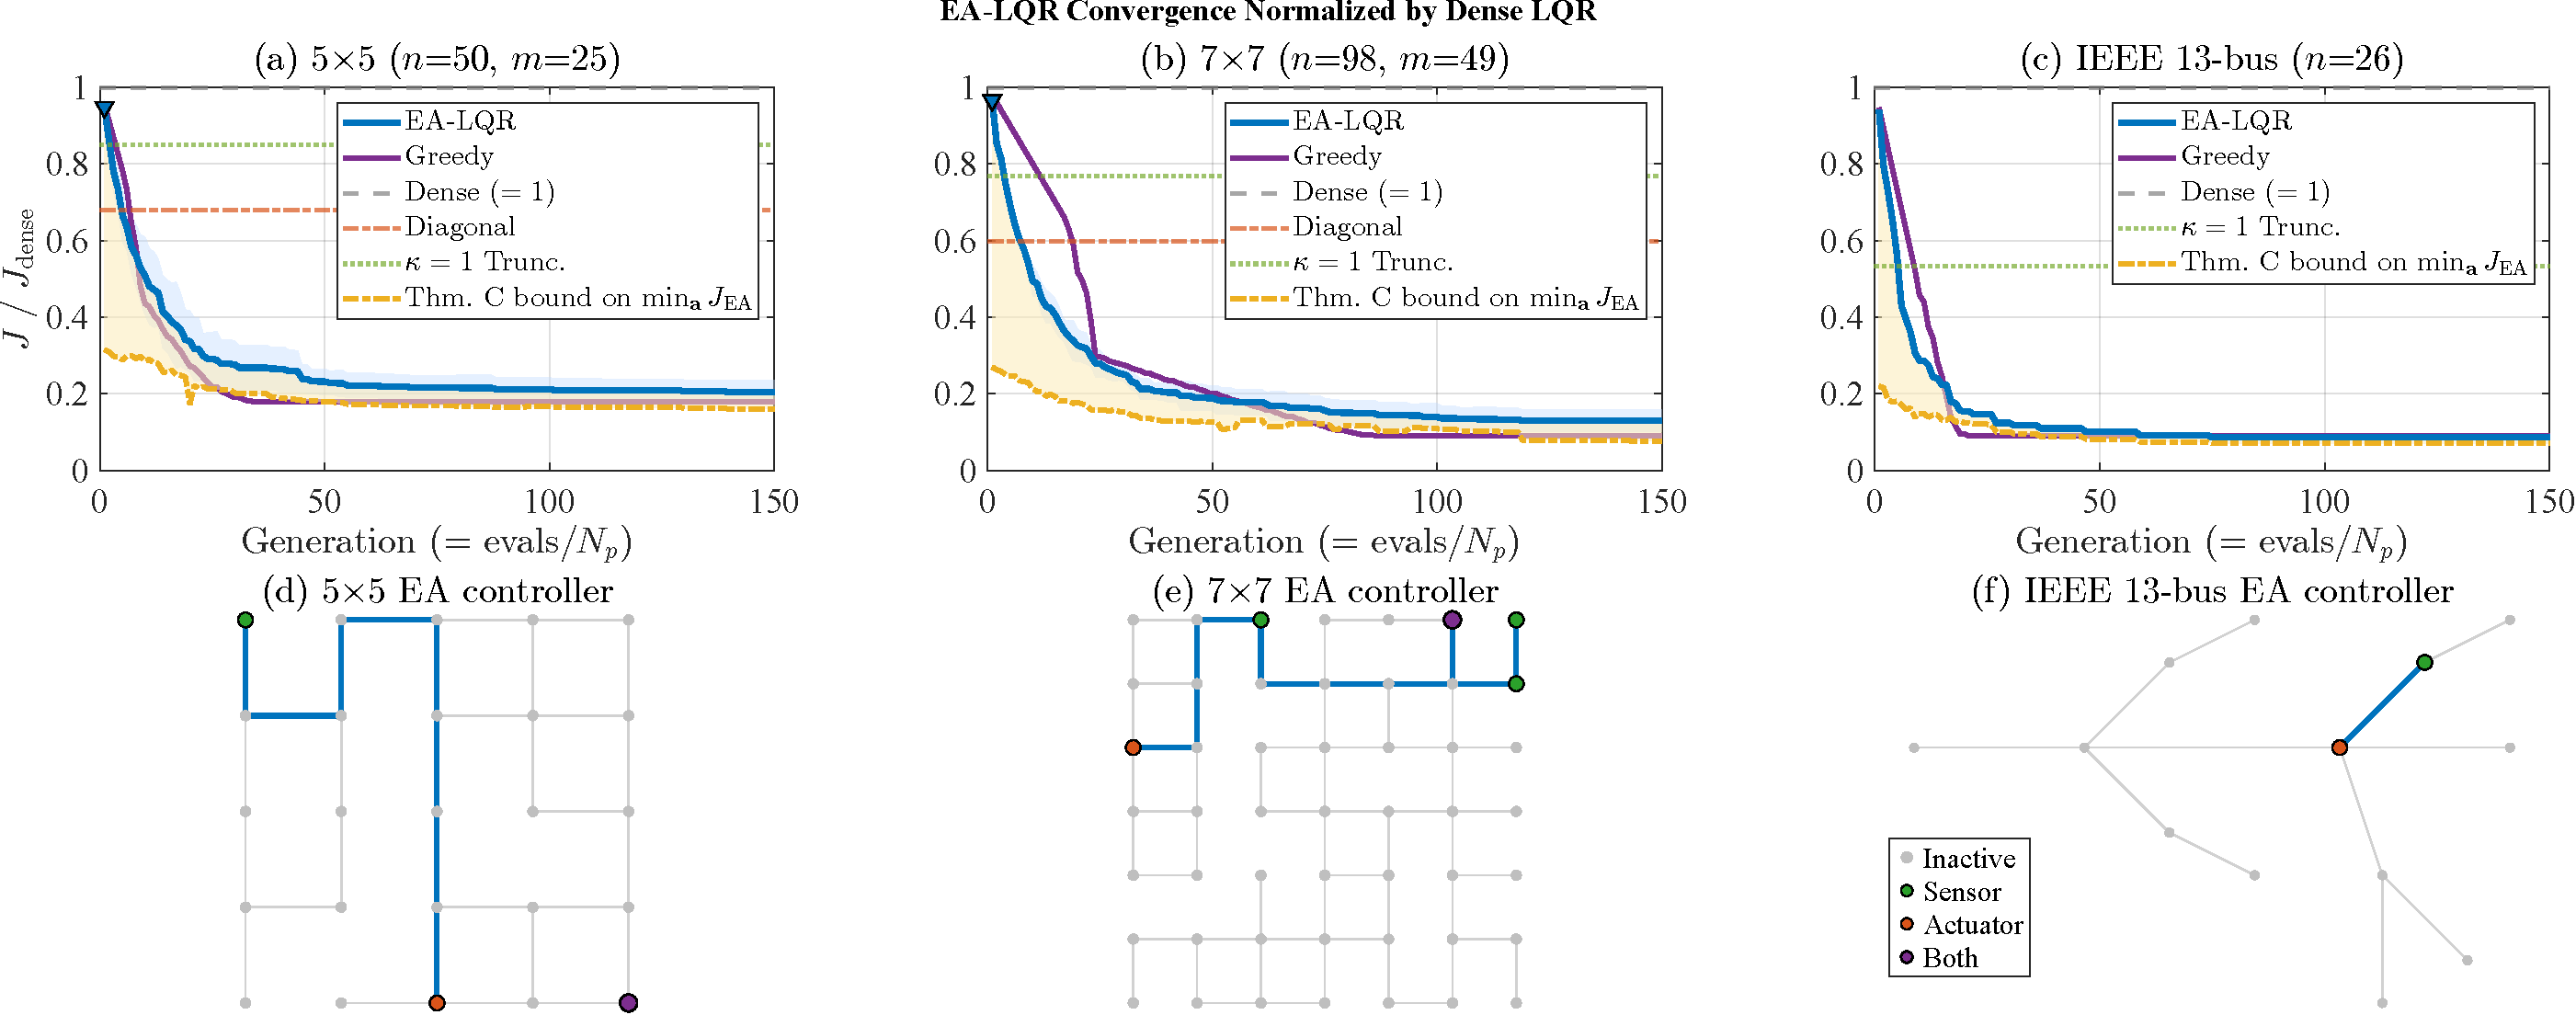
\includegraphics[width=\linewidth]{Fig1.pdf}
    \caption{Results of running Algorithm \ref{alg:ea} on three different plants, averaged over the three seeds $\{1,2,10\}$ of Table \ref{tab:greedy}. \textbf{Top panel:} normalized cost against a common budget axis --- Algorithm \ref{alg:ea} spends $N_p$ cost evaluations in the first generation and $N_p - n_e$ thereafter, so the greedy baseline is sampled at the EA's cumulative count. Normalized cost is $J_\mathrm{EA}(\theta^\star_t)/J_{\mathrm{EA}}(\theta_\mathrm{d})$, where $\theta^\star_t$ is the best gene of generation $t$. Solid blue: the EA, with $\pm1\sigma$ over seeds shaded. Solid purple: greedy. Dashed grey and red: the dense and diagonal LQR baselines; for the IEEE 13-bus system the diagonal LQR is unstable and is omitted. Dash-dotted amber: the certified lower bound of Corollary \ref{cor:gap}; the shaded band between it and the EA curve is the optimality gap over actuator masks at the elite's current $\ell$ and $\mathbf{s}$. \textbf{Bottom panel:} the controller returned by the EA at termination. Grey circles and dashes are plant nodes and edges; blue edges are communication links used by the controller; green, red, and purple circles are sensor, actuator, and combined nodes.}
    \label{fig:perf-conv}
  \end{minipage}
\end{figure*}

Next, we demonstrate the effectiveness of our proposed repair mechanism on an unstable system. We use the same $5{\times}5$ grid as previously, but scale plant matrix $A$ so that it has a spectral radius of $1.1$ and is unstable. We compare the performance of Algorithm \ref{alg:ea} alone with the performance of Algorithm \ref{alg:ea} in combination with repair mechanism Algorithm \ref{alg:gers-repair}, with parameter $\bar{\gamma} = 0.95$. We note that even without the repair mechanism, EA outperforms the baseline by about 44\%; however, with the repair mechanism, this improvement increases to 53\%. We also study the number of unstable individuals (as naively evaluated in Algorithm \ref{alg:ea} or evaluated after repair in Algorithm \ref{alg:gers-repair}). When no repairs occur, this values stays relatively fixed over generations; approximately half of the population is unstable at any given time. However, when repairs occur, early generations have nearly no unstable individuals. The number of unstable individuals rises in later generations, as the EA begins searching more and more sparse solutions that are more likely to be unstable prior to repair.

\begin{figure}[t]
    \centering
    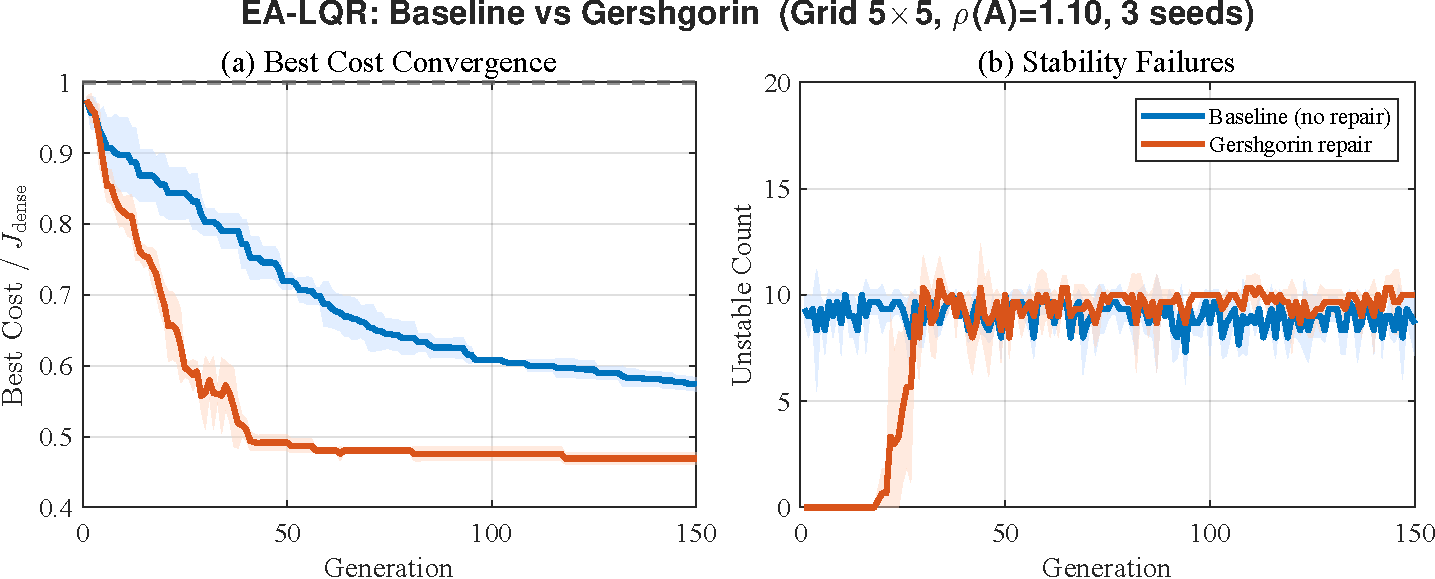
\includegraphics[width=\linewidth]{Fig2.pdf}
    \caption{Results of running Algorithm \ref{alg:ea} (``EA without repairs") and Algorithm \ref{alg:ea} with Algorithm \ref{alg:gers-repair} (``EA with repairs") on an unstable plant, averaged over three random seeds. Shaded regions indicate standard deviations. While both methods outperform dense LQR, the addition of Algorithm \ref{alg:gers-repair} further boosts performance.}
    \label{fig:gers_comparison}
\end{figure}
% ------------------------------------------------------------------------

% The full greedy subsection (Algorithm 3 float, fairness controls, architecture
% and unstable-plant discussion) lives in greedy_baseline.tex and is deliberately
% NOT \input here; only the summary, Table \ref{tab:greedy} and the scaling
% paragraph below are kept.

A greedy pruning search is the natural simpler alternative: it searches the same
gene $\theta$ through the same decoding and cost oracle, but only ever removes.
From the dense architecture it cycles three phases --- decrement $\ell$,
deactivate one actuator, deactivate one sensor --- each committing the single
best removal and never restoring anything, and stops when no removal improves
$J_\mathrm{EA}$. Neither search is charged for work it can prove redundant: the
EA reuses its elites' costs, and the greedy search skips a mask bit whose row or
column is already empty, since clearing it cannot change $K$. Both exclusions
are exact, and charging one but not the other would move the shared budget axis
by about a factor of two.

\begin{table}[t]
\centering
\caption{Final $J_\mathrm{EA}$, and the cost of getting there. The last column
is the greedy search's evaluation count divided by the EA's; it crosses $1$
between $N_u = 49$ and $N_u = 225$. The greedy search is deterministic; the EA
is not, and is reported as mean $\pm$ standard deviation over five runs where
five were run. The $15\times15$ row uses the length-scaled $p_m = 4/n$ and
$G_{\max} = 400$ of Remark \ref{rem:pm} rather than the $p_m = 0.05$,
$G_{\max} = 150$ of the rows above; at those settings the EA returns $84.7$.}
\label{tab:greedy}
\begin{tabular}{lrrc}
\toprule
Plant, seed & EA & Greedy & Ratio \\
\midrule
$5\!\times\!5$, 1   & $\mathbf{6.68 \pm 0.00}$ & $7.46$ & $0.13\times$ \\
$5\!\times\!5$, 2   & $5.81 \pm 0.12$ & $\mathbf{5.72}$ & $0.27\times$ \\
$5\!\times\!5$, 10  & $6.42 \pm 0.10$ & $\mathbf{6.33}$ & $0.21\times$ \\
$7\!\times\!7$, 1   & $6.35 \pm 0.83$ & $\mathbf{5.15}$ & $0.38\times$ \\
$7\!\times\!7$, 2   & $\mathbf{6.90 \pm 0.21}$ & $7.07$ & $0.45\times$ \\
$7\!\times\!7$, 10  & $8.64 \pm 1.11$ & $\mathbf{7.74}$ & $0.42\times$ \\
IEEE 13-bus, 1      & $\mathbf{2.45}$ & $2.55$ & $0.15\times$ \\
\midrule
$15\!\times\!15$, 1 & $12.73$ & $\mathbf{11.30}$ & $\mathbf{3.25\times}$ \\
\bottomrule
\end{tabular}
\end{table}

Finally, the two searches scale differently. In Fig.~\ref{fig:perf-conv} they
end within $1$--$3\%$ of each other, but greedy gets there sooner --- within
$2\%$ of its final value by generation $9$ on the $5\times5$ grid and $24$ on
the $7\times7$, against $48$ and $120$ for the EA. That ordering reverses with
size. Both pay $\Theta(N_x^3)$ per evaluation, so only the evaluation count
separates them. A best-improvement sweep costs one evaluation per live mask bit
and commits at most one removal, so the greedy search needs
$\Theta(N_u^2)$ --- intrinsic to steepest descent, not an artifact of our
implementation --- and we measure $0.26\,N_u^2$ at $N_u = 49$, $100$ and $225$
($630$, $2650$ and $13038$ evaluations). The EA's requirement grows far more
slowly, but only once $p_m$ is scaled with the gene length $n = N_u + N_x$ as
Remark~\ref{rem:pm} prescribes. On the $7\times7$ grid, $p_m = 1/n$ in place of
$0.05$ moves the elite from $7.01$ to $5.15$ --- exactly the greedy optimum ---
in $1510$ evaluations against greedy's $630$. On a $15\times15$ grid
($N_u = 225$, $N_x = 450$), $p_m = 4/n$ with $G_{\max} = 400$ reaches $12.73$
against greedy's $11.30$, within $13\%$ and on the same six actuators, using
$4010$ evaluations --- $31\%$ of greedy's $13038$. The crossover therefore falls
between these two sizes: greedy is the cheaper search on the plants of
Fig.~\ref{fig:perf-conv} and the more expensive one by $N_u = 225$.

\section{Conclusions and future work}
In this paper, we proposed an evolutionary algorithm to perform co-design of LQ control cost and material cost (actuators, sensors, communication links) on a linear time-invariant plant, and demonstrated its efficacy in simulations. While this paper focuses on the LQ case, the general proposed EA framework and repair mechanism may be applicable to nonlinear systems as well; this will be the topic of future investigations.

\bibliography{cit}
\bibliographystyle{IEEEtran}

\end{document}
